\section{Sakupljač otpadaka}
\label{sec:djubretar}

%Izvršavanje programa na računaru praćeno je stvaranjem brojnih struktura podataka (objekata).
%Neke od njih generiše sam program, dok su druge vezane za njegovu implementaciju. Sve te strukture podataka se skladište u deo memorije koji se naziva heap.

Strukture podataka koje su alocirane na heap-u a nisu dostižne preko nekog niza pokazivača programskih promenljivih, nazivaju se otpatci.
Memorija koju zauzimaju otpatci treba da bude dostupna za alociranje novih struktura podataka.
Taj proces se naziva \textbf{sakupljanje otpadaka} i događa se u fazi izvršavanja programa.

\subsection{Motiv}

Kod proceduralnih programskih jezika, kakav je na primer PASCAL,
operacije stvaranja i uništavanja objekata koji se skladište u heap-u izvršavaju se eksplicitnim navođenjem određenih naredbi (NEW i DISPOSE) u izvornom programu.
To znači da je odgovornost za recikliranje otpadaka na programeru, koji mora da svaki nepotrebni objekat uništi odgovarajućom naredbom i time oslobodi ćelije zauzete tim objektom.
Ukoliko to ne uradi kapacitet memorije se prividno smanjuje. Ova se pojava naziva oticanje memorije ili curenje memorije (memory leak). 
Ovakav koncept je prihvatljiv kod proceduralnih jezika, kod kojih su pomenute operacije retke, ali je neefikasan kada su u pitanju funkcionalni jezici koji se odlikuju čestim izvršavanjem tih operacija.
Zato je kod funkcionalnih programskih jezika posao sakupljanja otpadaka
(garbage collection) poveren delu sistema za upravljanje memorijom koji se naziva sakupljač otpadaka (garbage collector).

\subsection{Markirajući sakupljač otpadaka}

Ovo je najstariji tip sakupljača otpadaka. Razvijen je početkom 60-ih godina u
okviru programskog jezika LISP [Mcca60].
Programske promenljive i strukture podataka alocirane na heap-u formiraju usmeren graf.
Promenljive su koren tog grafa.
Čvor \textit{n} je dostižan ukoliko postoji put $r\rightarrow \dots \rightarrow n$ od nekog korena \textit{r}.
Pretragom grafa u širinu se markiraju svi dostižni čvorovi.
AKo čvor nije markiran, onda je otpadak, i treba da se realocira.
Čišćenje hipa se vrši počevši od prve adrese i ide do poslednje, traže se čvorovoi koji nisu markirani.
Dobijeni otpatci se povežu u listu (\textit{slobodnu} listu).
Tokom faze čišćenja takođe se odmarkiraju svi markirani čvorovi, da ne bi došlo do problema pri sledećem sakupljanju otpadaka.
Nakon što se izvrši sakupljanje otpadaka, prevedeni program nastavlja sa radom.
Kad god želi da alocira nešto na hip, dobija memoriju iz \textit{slobodne} liste. Kada slobodna lista postane prazna, to je znak da treba opet da se izvrši sakupljanje otpadaka.

\subsection{Sakupljač otpadaka sa brojanjem referenci}
\label{ref:reference counter}

Ideju za ovaj tip sakupljača otpadaka dao je Collins 1960.godine [Col60].
On se primenjuje u sistemima kod kojih je heap baziran na listi.
Svaka ćelija u heap-u sadrži jednu reč koja se naziva brojač referenci.
Vrednost te reči je broj referenci na ćeliju, tj. broj pokazivača koji na nju pokazuju.
Kada se neki podatak smesti u ćeliju i ona postane aktivna, njen brojač referenci dobija vrednost 1.
Ako u toku rada program kreira još neki pokazivač na tu ćeliju, njen brojač povećava vrednost za jedan.
Ukoliko se uništi neki pokazivač na ćeliju, brojač smanjuje vrednost za jedan.
Ako vrednost brojača postane nula, to znači da ne postoji nijedan pokazivač na tu ćeliju, tj. da joj se ne može pristupiti polazeći od nekog korenog pokazivača, pa ona više nije aktivna.
Čim ćelija postane neaktivna, reciklira se i to tako što se povezuje u listu slobodnih ćelija.
Ovim se izbegavaju dugotrajni procesi traženja aktivnih ćelija i recikliranja neaktivnih, koji su karakteristični za ostale tipove sakupljača otpadaka.
Sve ovo omogućava da se recikliranje otpadaka obavlja paralelno sa izvršavanjem programa, pa je ovaj tip sakupljača pogodan za real-time sisteme.

\subsection{Prepisujući sakupljač otpadaka}

Algoritam za ovaj tip sakupljača otpadaka dali su 1969. godine Fenichel i
Yochelson [Feni69].
Dostižni deo heap-a je usmereni graf, memorija su čvorovi, pokazivači su grane, promenljive su koren.
Prepisujući sakupljač otpadaka prolazi kroz deo grafa koji je alociran na heap-u, praveći izomorfnu kopiju u \textit{svežem} delu heap-a.
Taj sveži deo je kompaktan, i podaci zauzimaju kontinualan blok memorije, bez fragmentacije.
Koren sada pokazuje na kopiju a original se oslobodi.
\\
\\
Slika \ref{fig:copygc} prikazuje situaciju pre i posle prepisujućeg sakupljanja.
Pre sakupljanja, početni prostor je bio pun dostižnih čvorova i otpadaka, nije ostalo mesta za alociranje jer je dostignut limit.
Nakon sakupljanja novi prostor između alociranih čvorova i limita je slobodan za alociranje.

\begin{figure}[h!]
\begin{center}
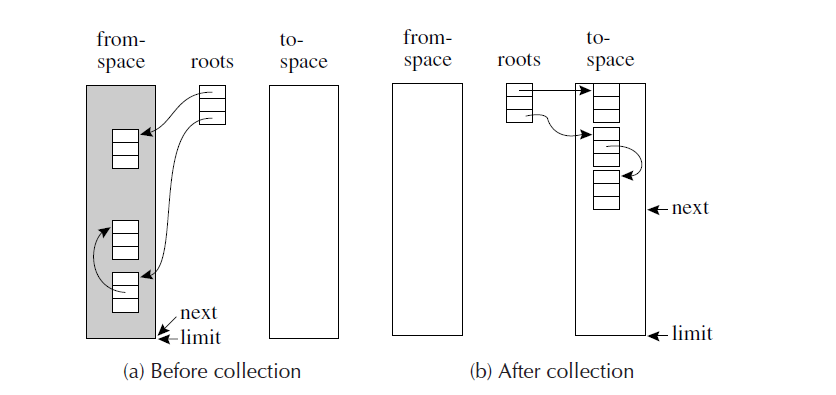
\includegraphics[scale=0.55]{copygc.png}
\end{center}
\caption{Prepisujući sakupljač otpadaka}
\label{fig:copygc}
\end{figure}

\subsection{Generacijski sakupljač otpadaka}
Jedna od mana prepisujućeg sakupljača otpadaka je što u svakom ciklusu
sakupljanja otpadaka premešta sve aktivne ćelije izvornog dela, odnosno objekte smeštene u njima.
To znači da će objekti koji imaju duži životni vek biti premeštani više puta, u toku više ciklusa sažimanja.
Ovo ponovljeno premeštanje predstavlja nepotreban posao, koji se može izbeći tako što će se heap podeliti na dva dela.
U jednom će se smeštati objekti dužeg životnog veka, što znači da će u njemu biti manje otpadaka, te će proces njihovog sakupljanja moći ređe da se vrši.
Drugi će sadržati objekte kraćeg životnog veka i zbog toga će imati veći broj otpadaka, pa će se kompakcija vršiti češće.
Strategija koja određuje koliko će se često neki region sažimati naziva se politika sakupljanja (collection policy).
\\
\\
Postavlja se pitanje kako odrediti koji objekti imaju duži životni vek, tj. kako odrediti koji će se objekti smeštati u koji deo heap-a. 
Empirijske metode su pokazale da većina mladih objekata (onih koji su skoro kreirani) predstavlja privremene strukture ili međurezultate, i da samim tim ti objekti imaju kratak životni vek.
Samo mali broj objekata je deo neke strukture dugog životnog veka.
U mnogim stilovima programiranja, kada se kreira objekat A, njegova polja se odmah inicijalizuju, i recimo da A pokazuje na objekte B i C.
Da bi to bilo moguće objekti B i C moraju već postojati, tako da imamo noviji objekat koji pokazuje na starije objekte.
Jedini način da stariji objekat B pokazuje na noviji objekat A je ukoliko je neko polje objekta B izmenjeno dugo nakon kreiranja samog objekta, što je empirijski mnogo retko.

\subsection{Odnos prema kompilatoru}

Kompilator za jezik sa sakupljanjem otpadaka uzajamno dejstvuje sa sakupljačem otpadaka generišući kod za alociranje podataka, opisujući lokacije za koren svakog ciklusa sakupljanja otpadaka i opisujući izgled podataka na heap-u (da li je lista, stek ili stablo).
Neki programski jezici i programi, veoma brzo alociraju memoriju na heap-u (i generišu otpatke).
Ovo je posebno istaknuto kod funkcionalnih programskih jezika, gde je obeshrabreno menjanje starijih podataka.


%% Osnovna referenca je Modern Compiler Implementation in Java, ANDREW W. APPEL

%% George E. Collins. “A method for overlapping and erasure of lists”
%% to je referenca za [Col60]

%[Mcca60] John McCarty, “Recursive functions of symbolic expressions and their computation by machine – I” The LISP Programming System

% [Feni69] Robert R. Fenichel and Jerome C. Yochelson, “A LISP garbage-collector for virtual-memory computer systems”
